% !TEX root = Thesis.tex

\section{Case Studies}

In order to expand on existing knowledge, a series of expert interviews has been conducted for this thesis. In the following section, the process of conducting the interviews is described. Next, there is an in-depth summary of each interview, concluded by an abstract to highlight the most important points for this thesis. The last section contains a comparison and evaluation of all interviews.

\subsection{Interview Technique}
%TODO evtl kürzer fassen
In order to complement theoretical findings from literature research, expert interviews have been conducted. A structure for the interviews has been defined (see appendix). In this way, statements from different experts can be compared and evaluated, which allows for a comprehensive review. Even though interviewees may share their native language (German) with the interviewer, interviews have always been conducted in English. Thus, any inaccuracies that may occur during translating the statements were prevented and comparability of interviews has been improved.

The interviews were held remotely, either via an Internet VoIP-Service such as Skype, or via using WebEx, the standard communication platform used at T-Systems when interviewing employees of this company. Considering the often tight schedules of experts in their fields, the duration of interviews was planned to be 45 minutes.

To further document the interviews and the steps leading up to them as well as the steps of refinement that follow, a process (see figure \ref{fig:Intprocess}) has been defined and adhered to. 

\vspace{3mm}
\begin{figure}[htb]
	\centering
	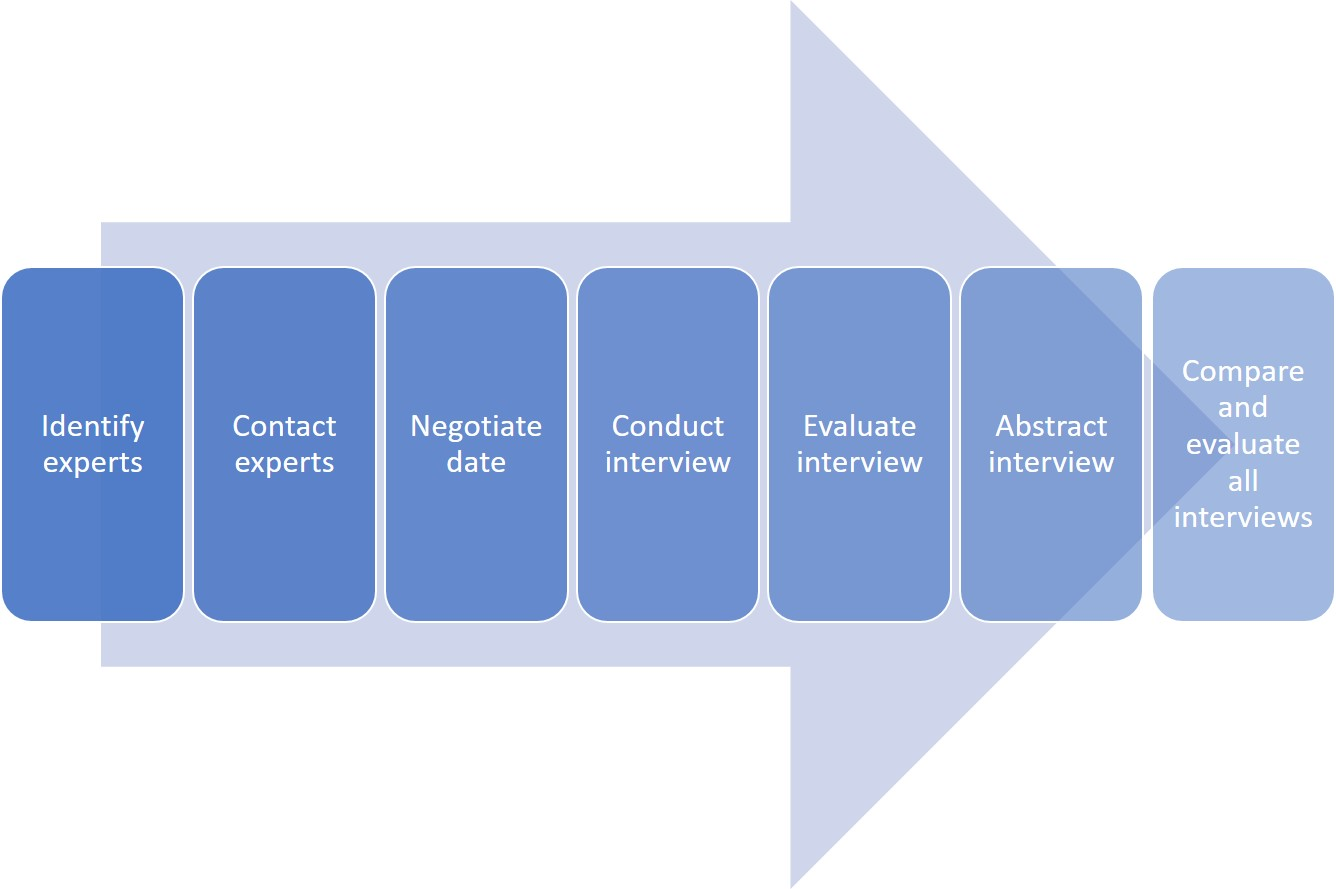
\includegraphics[width=0.85\textwidth]{Pictures/Interview_process}
	\caption{Interview process}
	\label{fig:Intprocess}
\end{figure}

\newpage

\paragraph{Identify experts} The experts are identified by conducting a network-based search. Initial contacts are asked to identify persons they consider an expert on the topic, who are in turn asked to provide further contacts.
\paragraph{Contact experts} Initial contact to the expert is established via an email sent by the expert's contact. Included is a standard email explaining the topic, duration and process of the interview and providing the researchers' contact details.
\paragraph{Negotiate date} Once the expert has agreed to participate in the interview, the researcher contacts them directly in order to set up date, time and method of communication for the interview. Note that all interviews are conducted using at least voice-based communication. Video can be added to further facilitate the communication between the expert and the researcher.
\paragraph{Conduct interview} The interviews are conducted in five phases with defined leading questions\footnote{The structure of the interview can be found in the appendix, page \pageref{app:InterviewStructure}.}. This means, the leading questions will be asked, but the researcher will also ask further questions as appropriate to the course of the interview. These phases are:
\begin{itemize}
	\item Introduction
	\item Offshoring Experiences in the USA
	\item Offshoring Experiences in Germany
	\item Comparison of Experiences in Germany and the USA
	\item Finalization
\end{itemize}
During the interview, audio has been recorded. The audio files form the primary source of knowledge gained from the experts.


\paragraph{Evaluate interview} The recordings are evaluated and any important passages are noted. These evaluations are added to the appendix.

\paragraph{Abstract interview} For each interview, an abstract is developed. The abstracts are included in the thesis.

\paragraph{Compare and evaluate all interviews} Finally, an overview and comparison of all interviews is generated to derive common statements and areas of disagreement.

\newpage
\subsection{A German Project Manager on Offshoring with Different Service Providers}

This interview was conducted on 1. July 2016 08:00 h CEST with Michael Scheitza, a senior project manager at T-Systems International. The standard communication tool of T-Systems, Cisco WebEx, was used for the interview. The recording of the interview can be found on the enclosed CD (file name: 20160701\_Michael\_Scheitza.mp3). A written summary of the interview is found in appendix, page \pageref{int:Scheitza}.

\subsubsection{Background}
Michael Scheitza has worked for eight years as a project manager in an international environment. He has experience in offshoring projects with Russia, Poland, Romania, India, Malaysia, Mexico, and Brazil. He does not have any experience with offshoring from a U.S. perspective, so he did not feel comfortable answering any questions regarding this topic. 
\subsubsection{Results of Interview}
At T-Systems, application management contracts are often delivered offshore. Most customers leave the choice of delivery location to T-Systems, provided there is no legal obligation to deliver locally. The delivery model for each contract is chosen by the necessary skills, the language that is requested by the customer, and required service levels. When deciding on a delivery location, scalability is very important. It is essential that there are enough people with the required knowledge.

Generally speaking, there are two different possible working relationships between customer, German on-site team and offshore team. %Bilder hier einfügen

\vspace{3mm}
\begin{figure}[htbp]
	\centering
	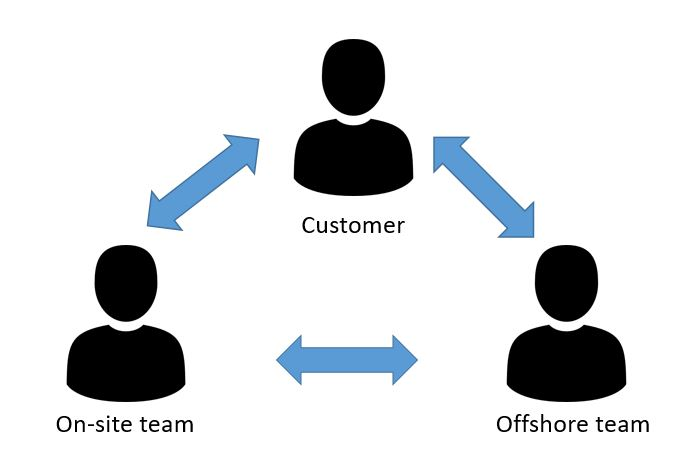
\includegraphics[width=0.5\textwidth]{Pictures/1on1_relationship}
	\caption{Direct, personal relationships between customer, on-site team and offshore team}
	\label{fig:1on1}
\end{figure}

The first possible working relationship works best in teams smaller than 50 persons offshore. In the transition phase, offshore team members travel to Germany in order to directly interact with and learn from the customer. In figure \ref{fig:1on1}, the set up in this case is depicted.

The interviewee gave an example of an application management contract that was delivered from Brazil. There was the requirement that all 20 team members speak enough German to directly speak to the customer. In transition phase, personal relationships were established between the Brazilian team, the customer and German project management of T-Systems. This facilitated collaboration later in the project, because the persons involved knew each other in person, not only via telephone and email.

The motivation for the offshore team in this case stems from the identification as part of a global delivery team. If the on-site and offshore teams share the same tasks, the delivery model is called \textit{Verl\"angerte Werkbank}. The team size in this case is usually less than 30 people and the project manager distributes tasks directly to offshore team members. 

The drawback in this approach is that it tends to increase volatility in the team. Michael Scheitza shared an experience he made with an Indian team: Each time there were quality issues, T-Systems had spent money on bringing team members on-site or German project management had traveled to India to improve communication. Few months later, he noticed that especially those team members who had been to Germany left the project and changed jobs in order to further their careers. This way, the investment in communication was unsuccessful.

\vspace{3mm}
\begin{figure}[htbp]
	\centering
	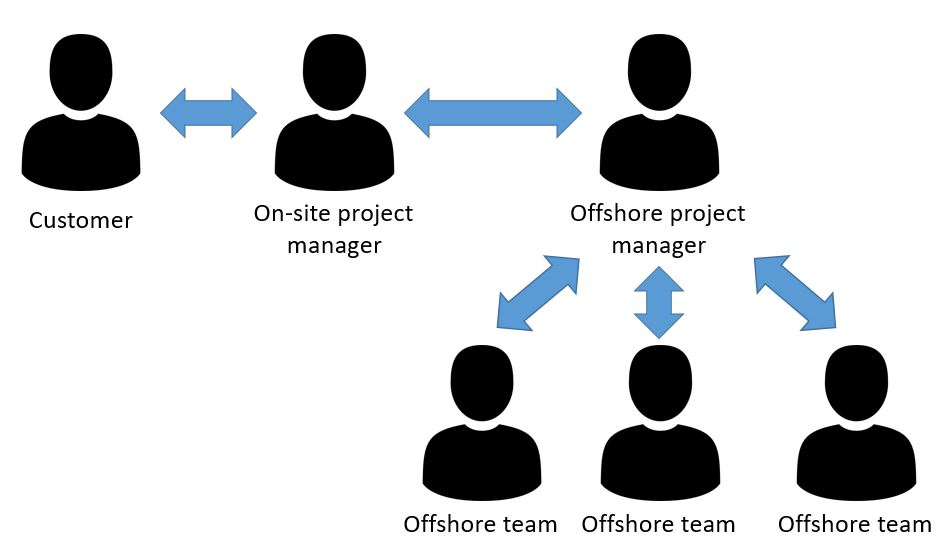
\includegraphics[width=0.7\textwidth]{Pictures/Hierarchy}
	\caption{Hierarchical communication between customer and offshore team}
	\label{fig:hierarchy}
\end{figure}

The second possibility is used in larger teams with more than 50 people. Teams that size are large enough to be organized in hierarchical layers with a local team lead or project management. This approach does not involve deep relationships and personal communication. Instead, the working relationship is managed via \glspl{sla} and \glspl{kpi}, where quality and quantity of deliverables are defined. The communication structure in this case is depicted in figure \ref{fig:hierarchy}. In transition phases of projects, only the offshore project managers or team leads travel to Germany and distribute the knowledge they gained in working with the customer to their teams offshore.

In this case, the offshore team does not identify as a part of a global delivery team, because the personal relationships that are needed for this approach are not in place. Alternately, the team members can identify with the project itself and are motivated by the local project manager. Ideally, the team is driven by the desire to be successful in fulfilling the contract.

Neither approach, said Michael Scheitza, is clearly superior to the other. Each has its drawbacks and advantages, and both are applicable in certain situations.

\subsubsection{Conclusions}

In the interview, Michael Scheitza differentiated and specified two distinct approaches to offshoring that are used in Germany. In table \ref{tab:ScheitzaApproaches}, they are directly compared to each other. 
\vspace{3mm}
\begin{table}[htb]
	\centering
	\begin{tabular}{l|p{5.8cm}|p{5.8cm}}
		& \textbf{Personal Relationships} & \textbf{Numbers-based Approach}\\\hline
		
		\rule{0pt}{3ex}Team size &$<$ 50 people &$>$ 50 people\\ \hline
		\rule{0pt}{3ex}Transition phase&All offshore team members travel on-site and form personal relationships with T-Systems team members and customers &Offshore project managers travel on-site and share their knowledge with the team\\ \hline
		\rule{0pt}{3ex}Communication &Direct communication between customer, on-site team and offshore team & Hierarchical communication from customer to on-site team to offshore project management to offshore team \\ \hline
		\rule{0pt}{3ex}Motivation &Identification as part of a global delivery team &Motivation by local project management and identification with the contract \\ \hline
	\end{tabular}
		\vspace{3mm}
		%Immer caption vor label!!!
		\caption{Comparison of German offshoring approaches according to M. Scheitza}
		\label{tab:ScheitzaApproaches}
\end{table}

Even though the interviewee could not contribute any experience with offshoring from an American point of view, there have been very interesting points. Firstly, the other interviews focused mainly on offshoring with an Indian service provider. This interview offered insights in offshoring projects with a multitude of different destinations. Secondly, there were criteria for choosing a delivery model outlined. Last, the two different collaboration models were described very thoroughly, offering a concise view on the offshoring projects the interviewee experienced.


\subsection{An Indian Offshoring Pioneer Comparing German and U.S. Clients}
A. S. Viswanathan agreed to be interviewed on 7. July 2016 at 17:00 h CEST / 20:30 h IST. For this, Skype was used as a communication tool. On the enclosed CD, the recording of the interview has the file name 20160707\_A\_S\_Viswanathan.mp3. The summary of the conversation can be found in appendix page \pageref{int:Viswanathan}.
\subsubsection{Background}
The interviewee is electrical engineer with a specialization in industrial engineering. In 1978, he started his career with English Electric, which was a part of General Electric Group. There, he worked for two years before joining Siemens. With Siemens, he held various positions ranging from the shop floor to CIO of the IT subsidiary of Siemens in India. Later, he moved on to the board of Siemens Information Systems, a software company that took global mandate within the Siemens Group. His responsibilities included Business Solutions for offshoring SAP, which his team was pioneering in India, as well as IT services.

In 2007, Siemens merged all local IT companies into a new company called IT Services and Solutions. Viswanathan was on the executive management of this company, heading Global Portfolio of Mobility.

After taking a break in 2011, he founded his own management consultation company in 2012. He specializes in offshoring consulting, primarily with customers from Germany, China and India.

\subsubsection{Results of Interview}
\paragraph{Offshoring in the U.S.}When first conceptualizing the offer of offshoring services, the first customers were from the United States. They were very quick in understanding the advantages and seizing the opportunity, not only shifting single tasks, but entire operations to India. Before offshoring, U.S. companies took the time to evaluate different service providers. Once the decision was made, there was no plan B, so there was a necessity to make offshoring work.

This has a profound effect on working relationship. In Viswanathans experience, contributing to positive working relationships was English being a common language. Management meetings and schedules were easily set up. \Glspl{sla} were more critical, as after the initial cycles of new contracts, there would be a new wave of requirements, imposing stricter quality standards. In this phase, facts and figures dominate the working relationship.

The American approach to offshoring is characterized by legalistic and contractual concerns. When researching service providers, U.S. companies have consultants performing background searches of companies providing operations in India. Three to four companies are shortlisted and visited by the American team for presentations. Thereafter, contract negotiations start. A lot of emphasis is placed on contracting and commercial \glspl{sla}. The processes are not deemed as important, since the companies believed in the ability of the service provider to deliver.

Contributing to the success of American offshoring projects is the high offshorability of an American job. The work is conceptualized as a specific set of tasks where a specific set of skills is needed. Therefore, the skills of workforce can easily be managed. This goes back to U.S. companies already have experience with shifting jobs within the U.S. and people are already working in different places and time zones within the country. Also, jobs are very transaction-based in the U.S.. The education system facilitates that each employee does not need to have an end-to-end knowledge of the entire process. This is connected to the higher fluctuation of employees in American companies and is a huge advantage when it comes to offshoring -- it needs only minimal training to enable a new person to do the job.

\paragraph{Offshoring in Germany}Compared to American jobs, in German companies the job design is much more intrinsic and process-oriented. An example of a buyer is given: in Germany, the buyer has a specific background in the field, maybe an apprenticeship or some other kind of special training, whereas the buyer in the U.S. is not expected to have deep insights in the field when starting the job. The German buyer has knowledge in costing, the market, and product design, whereas the American buyer consults a technical specialist for those details. This system-oriented thinking is an advantage for the German society, but an obstacle for offshoring.

This kind of job design is mirrored in the SAP systems of companies. When it comes to customizing the system, a German system differs greatly from an American system, because the role of an individual is more holistic in Germany. This presents a problem when shifting tasks offshore, as one person in Germany can't simply be replaced by one person in India as it is the case with American jobs. The person in India simply lacks the specific background and experience with the German company.

Furthermore, offshoring is a very alien concept for German companies, especially \gls{sme}. Those grow very organically from small family businesses, so the owners have in-built control of all processes from the beginning. When it comes to outsourcing within Germany, the service provider does not have full control of the entire process, but only provides some parts. Additionally, German service providers often have a very good knowledge of their customers, and are almost an extension of their customers' organization. 

When it comes to offshoring, both of these points present problems. When relocating tasks, the customer inevitably needs to give up control over processes. Similarly, when replacing domestic outsourcing with an offshore provider, the same standard can not be applied to a foreign company that is used to evaluate a German company that has years of experience collaborating with the customer. Additionally, Germans tend to display a high degree of detailing, so the standards for the service providers are often very high. This has, in Viswanathan's experience, been one of theo biggest barriers for German companies approaching offshoring, and it is important to achieve a change in mindset for this. Also, in general Germans are more used to exporting than to importing. The notion to import services from a different country is somewhat foreign, as it implies that the service provider could do the job better than the German company itself.

It is very typical of German companies to prefer \gls{fdi} over foreign outsourcing. Frequently, an implicit objective is recreating the own organization in India. The reason for this is the inability of German companies to change the structure of jobs in a way that makes them easily offshorable.

Language is a further important point that must be discussed when talking about offshoring in Germany. German companies are becoming more international, but many still prefer to have their systems built and maintained completely in German. This is becoming less of a problem as many Indians are learning German, but it still is a handicap.

Additionally, the transition phase must be carefully managed when implementing offshoring, especially with respect to the loss of jobs or the decrease of job security in the German company. Work councils and unions make this process slow and difficult. This needs to be accepted and accounted for in the planning both on the German and Indian side. A comparable American company would be much quicker in implementing offshoring, which is a tremendous disadvantage for German companies. In the worst case, Viswanathan recounts, shortly before completing the transition, unions had objected to an offshoring project so all measures had to be reversed. This was a very difficult scenario for both the service provider and the customer, as the setup in India was already completed.

A German company that wants to offshore successfully first needs to define entire functions that can be offshored, rather than offshoring just some minor roles. Second, if the company is looking to offshore not only easily offshorable IT services\footnote{Hardware, infrastructure support and similar tasks}, but business processes, they must be designed in a way that the transactions are separated from the decision-making. Then, the transaction part of the job can be offshored without many problems. However, as long as jobs are looked at in an integral way, it is an obstacle to offshoring. The very deep level of job ``slice and dice'' that is common in American jobs is not needed, but that one level of division could help German companies to more success in offshoring.

Application management is identified as one function that is easily offshorable. In general, the tasks could be dealt with replacing one German resource with three Indian resources. This, of course, results in a much smaller cost arbitrage but still yields an economic advantage as multitasking can be applied in the Indian site. The distribution of work is managed by Indian managers who have enough knowledge of the entire process in this scenario. Obviously, this is a lot more management effort than offshoring with an American companies would entail.

\subsubsection{Conclusions}
In this interview, Viswanathan described the very different experiences he had with German and American clients. Many of his points are supported by literature research as laid out in section \ref{sec:Theory}. To recap his statements, in table \ref{tab:ViswanathanComparison} the German and American approach to offshoring according to A. S. Viswanathan are analyzed.

\vspace{3mm}
\begin{table}[htb]
	\centering
	\begin{tabular}{l|p{5.55cm}|p{5.55cm}}
		& \textbf{U.S.} & \textbf{Germany}\\\hline
		\rule{0pt}{3ex}Job design& Transaction-based, no need of end-to-end process knowledge, specific set of tasks with deep level of  &Holistic, process-oriented task which require extensive domain knowledge\\ \hline
		\rule{0pt}{3ex}Employee education&Minimal training &Specialized vocational training, apprenticeship or academic background and years of experience in the company \\ \hline
		\rule{0pt}{3ex}Offshoring approach&Contractual and legalistic focus when setting up offshoring; Emphasis on \glspl{sla} &\gls{fdi} is preferred in order to recreate the own organization in the offshoring destination \\ \hline
		\rule{0pt}{3ex}Expectations&Quality is adjusted in multiple waves of requirements &Very high quality standards from the start\\ \hline
		\rule{0pt}{3ex}Shifting ratio& One American resource to one Indian resource & One German resource to three Indian resource\\ \hline
		\rule{0pt}{3ex}Language&Facilitates communication and collaboration &Rare skill offshore, hard to learn \\ \hline
	\end{tabular}
	\vspace{3mm}
	%Immer caption vor label!!!
	\caption{A. S. Viswanathan's comparison of American and German approaches to offshoring}
	\label{tab:ViswanathanComparison}
\end{table}

As shown in the table, German companies in comparison to American have quite a few obstacles to overcome in order to successfully offshore. Some of the characteristics that are unique to German companies and have often proved to be an competitive advantage in global markets are at the same time a disadvantage for offshoring. The most important point is here the difference in job design. 

A. S. Viswanathan provided the vast knowledge and experience with offshoring he has gained over the course of his career in this interview. In a pointed way, he determined the differences of American and German companies when it comes to offshoring. Having worked with both American and German clients, he is in a unique position for making this comparison.

\subsection{A German Global Delivery Expert on FDI Experiences}
The interview with Ingo K\"ummritz took place on 04. August 2016 at 10:00 h CEST. As a communication tool, Skype was used. The file name of the audio recording on the enclosed CD is 20160804\_Ingo\_K\"ummritz. The written summary is in appendix, page \pageref{int:Ingo}.

\subsubsection{Background}
Ingo is German, but went to High School and College in the U.S., which has helped him broaden his horizon when it comes to international delivery. In 2003 he was working at IBM and the country manager approached him, offering him to take responsibility for global delivery. In this time, he was in the role of a principal, which is a topic expert within the IBM organization. Later, after 10 years of working at IBM, he switched jobs and started with Siemens, moving to a customer-facing role. Several years later, he had a short contract at an Indian company and ended up at NTT Data in Germany afterwards. At present, he holds a subject matter expert role again.

All in all, Ingo has been working in the area of global delivery for 13 years, mostly with India. In this time, he was responsible for large projects and \gls{ams} deals in delivery, sales, and customer-facing positions. This has helped him to understand all partners involved better. In offshoring projects, he has been both in integrated delivery teams and in customer teams that traveled to India to set up offshoring there. His experience pertains to \gls{fdi} only. Whenever he has worked with an Indian team, they were his colleagues at IBM or Siemens.

Even though he does not have first-hand experience with offshoring from an U.S. perspective, he spent quite some time there and had many American colleagues, considering IBM is an American company. In a way, the work they did at the German subsidiary of IBM could be considered offshoring by the American headquarter.

\subsubsection{Results of Interview}
When talking about global delivery, there is no dedicated location for delivery, but rather a delivering company. This company needs to find the right delivery model with regard to resources and locations. The right location is not necessarily India, but this country is the global powerhouse in the \gls{ict} industry. About 90\% of the projects and services that included offshoring in Ingo's experience involved the Indian subsidiary. The time zones are very convenient for offshoring, as well, because Central European business hours can be covered from India without needing to use late shifts.

The critical point, regardless of the type of work that is being offshored, is communication and cooperation. It is critical to learn how the counterpart on the service provider side is thinking and reacting to communication. Rather than processes, methods and tools, interaction is the critical factor in offshoring. Still, the right processes, methods and tools are the basis for successful work in Germany or in an international context.

\paragraph{Offshoring in the U.S.}
There are two main drivers to offshoring in the U.S., to Ingo's knowledge. One of those drivers is the cost arbitrage between employing Indian and American administrators or IT engineers. In U.S. companies, the willingness to take risks in order to take advantage of this is generally quite high when compared to German companies. The second driver is for companies not involved in the IT industry, there is often a high volatility in the business behavior. There need to be large teams set up on short notice and the hiring process takes just too long in the U.S., especially when the needed skills are uncommon. Instead, the company shifts the tasks offshore. For example, DHL used to employ 4000 Indians from Infosys, an Indian-based company, in the U.S.. Then, after Deutsche Post bought the company, service providers were consolidated and did not include Infosys any more. This shows the different approach to offshoring of German and American companies. Business plans of new ventures in the U.S. almost always include out-tasking certain areas.

Supporting this willingness of American companies to offshore is the tendency of having a much higher tolerance for software code that is not 100\% perfect, but performs fast, than engineering-oriented civilizations such as Germany, Switzerland, or Nordic countries. This is a sign of a dedication to get new products to the market quickly. American companies are not as concerned about failures as German companies. If a new product fails at an American company, they analyze the mistakes that have been made and start over, whereas German companies try to avoid failures.

But there is not only a demand of American companies seeking to offshore, but also a supply of Indians that like to be working for American companies. Indians have adopted the American way of building their career and CVs based on the reputation of their employers, so they love to join Indian subsidiaries of companies like Dell, HP, IBM, Accenture, or one of the top-tier Indian service providers like Infosys. Also, there is no language barrier between the U.S. and India,  as English is an official language in India. Both of those factors contribute to the low barriers American companies face when setting up offshoring.

When it comes to working relationships between American companies and their service providers, there are two main possibilities. The first is a numbers-based approach, where the tasks are handed over and the service provider is managed like a subcontractor, so there is not much of an involvement on a technical or personal level. The other is the approach of building an integrated team. In this three-tier delivery model, on-site staff, people from India on-site and people offshore are working together with defined roles and rotations. Working in this way builds more of a partnership between the customer and the service provider. Both of these approaches work well in the appropriate circumstances. From the customer's perspective, there is also the additional possibility of hiring a global delivery company and collaborating only on a strategic level. The service provider then decides on delivery model and locations.

American companies are better at utilizing dedicated offshore centers. Those are dedicated teams offshore that are reserved for a certain customer. When this customer is an American company, they will get very creative in finding extra work for the offshore team to keep them occupied. In this way, tasks that keep getting postponed because there are more urgent issues at hand will be completed, even if those tasks are not in the initial scope of the offshoring project. American companies approach offshoring centers with a certain level of trust and are willing to pay for the reserved manpower in case something urgent needs to be done. 

An example for this is when Ingo was working for IBM, he needed some Indian SAP experts for an upcoming project. He approached the head of the SAP resources in India, he was told there was no one available, because of the 250 people with the required skills, 50 were in existing projects, and 200 were reserved by the American part of IBM. So Ingo could not get anyone for his project, and he thought that it was incredible to have such manpower on the bench, waiting for new projects. Nobody from the German part of IBM was willing to operate likewise, ramping up an Indian team months in advance in order to be able to engage once a new project started.

\paragraph{Offshoring in Germany}
When offshoring started to take off in Germany, there was a myth about offshoring in India that Indians are great and able to deliver any task, based on only the requirement documentation. Of course, there are many highly-skilled professionals in India, and of course, they will deliver when given a task, but that does not imply that all projects where something is delivered are successful. German companies, in the beginning, approached Indians as they would a German factory worker, handing over documentation and checking for results a few weeks or months later. This does not work with India.

So German companies needed to learn how to deal, on a partnership level, with Indians. The first attempts were talking to the service provider once in a while during the projects. When the Indian colleagues were asked if they understood the documentation, they assured that they did, but the projects still failed.

The next wave of learning included trying to understand the cultural background of the Indian colleagues better. When asked to perform a task, they would confirm they could do it because they did not want to fail their customer, regardless if they could actually deliver or not. A German would protest if they could not complete a task because of missing skills or a too small time frame, so German companies assumed Indians would do the same.

Once German teams learned how to hand over tasks to India, check for results and employ trust, they could build an integrated team with the Indian colleagues. With this approach, projects succeeded, and the integrated teams continued to succeed for a long time, because the mutual level of trust and understanding was a great motivation for all participants.

From the Indian side, service providers have made the effort to understand their German customers better, as well. They founded small centers in Germany and hired local people who could make a bridge between India and Germany, in order to be more successful in Germany.

Of course, language is an important factor when talking about offshoring in Germany. Volkswagen, for example, insists on their IT systems being built and managed completely in German. Additionally, they place a lot of emphasis on project teams being directly on-site their headquarters in Wolfsburg. So for a multi-million euro project there are 150 IT engineers needed, of which 100 need to be fluent in German. This creates huge problems with staffing. BMW, on the other hand, is more international and even requires Chinese in some German positions. The Chinese market has become very important for them.

Many Germans, especially the demographic over 45 years, are not very confident in their English skills. They know the language, but they fear making mistakes when using it, particularly in spoken communication. This creates the feeling that they are exploitable and their communication partner will use this weakness to win negotiations. The only way to improve this insecurity is exposing people to situations where they can use the foreign language without high stakes or pressure.

When trying to set up \gls{fdi} in India, many German companies face the problem that they do not have a brand in India and are not known by the general public. This is an obstacle in attracting enough skilled resources for new offshore centers.

German companies, compared to American companies, are hesitant with using dedicated delivery centers. They do not want to pay for 100 people when the tasks in scope only require 20. This hesitation might stem from a lack of trust on the German side. Also, Germany generally has a risk-avoiding culture which may be aggravating this. Risk-avoiding in this context does not mean that no risks are taken, but German companies have a tendency to perform several rounds of risk-assessment and the need to collect as much information as possible in order to correctly evaluate risks before they are accepted.

Meeting culture in Germany is based on a round-table mentality: everybody gets to contribute their opinion on an upcoming decision. This often prolongs the decision-making process. On the other hand, the quality of decisions in German companies is often very good, as many people have contributed their knowledge.

Germany is a society where an engineer approach to problems is deeply ingrained in the culture. There is a desire to learn why something does not work. As the first bank institutions ran into problems when they started offshoring, they found that their local experts did not get as much relief as anticipated, because offshoring came with additional management overhead. When they switched to integrated teams, they could reduce the communication gap and increase the success rate of projects. Many German companies have gone through the same learning process since, and most have arrived at the integrated team approach as the most successful delivery model.

German companies have needed a long time and lots of experience to learn how to implement offshoring, to use checks and balances, to have a communication plan and how to deal with the Indian colleagues. Once these are in place, offshoring can work very well for a long time in German companies. Ingo's key statement is: ``If you are capable of combining German engineering and Indian enthusiasm, then you have a successful team.''

\subsubsection{Conclusions}

Ingo outlined in his interview the main points that help American companies in achieving offshoring success, and contrasted them to the obstacles German companies face when trying to set up offshoring. His statements are summarized in table \ref{tab:IngoComparison}.

\vspace{3mm}
\begin{table}[htb]
	\centering
	\begin{tabular}{l|p{5.2cm}|p{5.2cm}}
		& \textbf{U.S.} & \textbf{Germany}\\\hline
		\rule{0pt}{3ex}Offshoring approach&Numbers-based or integrated team approach &Mainly integrated teams \\ \hline
		\rule{0pt}{3ex}Willingness to take risks& High & Only after several rounds of risk assessment \\ \hline
		\rule{0pt}{3ex}Maturity &High & Learning process about communication and cultural backgrounds \\ \hline
		\rule{0pt}{3ex}Employer brand&Very desirable &Mostly unknown \\ \hline
		\rule{0pt}{3ex}Main drivers&Cost arbitrage and high business volatility &Cost arbitrage \\ \hline
		\rule{0pt}{3ex}Decision making &Prepared by specialists & Round table process \\ \hline
		\rule{0pt}{3ex}Language &English is an official language in India & Limiting factor for availability of resources \\ \hline
		\rule{0pt}{3ex}Resource using &Dedicated offshore centers reserved for one customer, will be used for work backlog if no projects are running& Pay-per-use model\\ \hline
	\end{tabular}
	\vspace{3mm}
	%Immer caption vor label!!!
	\caption{Insert caption here}%TODO
	\label{tab:IngoComparison}
\end{table}

For German companies, Ingo sees a lot of obstacles when it comes to offshoring. In his experience, once a company has completed the learning process and checks and balances, a communication plan and mutual understanding are in place, it can benefit greatly and over a long time span from offshoring.

The following action items can help German companies to improve their offshoring potential:
\begin{itemize}
	\item Internationalization of systems and processes
	\item Encouraging employees to learn and use the English language
	\item Using and utilizing offshore centers
	\item Making an effort in understanding the cultural background of the new colleagues
\end{itemize}

Talking to Ingo offered deep insights into the differences in German and American offshoring ventures that were often illustrated with examples. Even though in his experience, German companies face many obstacles, he provided action items that could help them improve their offshoring processes.

\subsection{Subir Purkayastha}
Subir was interviewed on 06. August 2016 at 10:00 h CEST / 17:00 CST via Sykpe. The written summary of the interview is in appendix page \pageref{int:Subir}. The recording can be found on the enclosed CD, file name: 20160806\_Subir\_Purkayastha.mp3.

\subsubsection{Background}

After completing his undergraduate studies in engineering back in India, Subir went to the U.S. for graduate studies, initially in engineering. Afterwards he worked for a few years, before going back to graduate studies. He completed a PhD-degree in a Computer Science related field at the University of Michigan.

For 15 years, he worked at AT\&T Bell Labs, where he developed network software products. Then, he joined Siemens, where he headed the telecommunications business unit in the IT division of Siemens India. In the duration of his employment, Siemens built up the software division in India from 150 to 7000 people. In his business unit, he managed about 500 people and a revenue of 100 million dollars a year, working extensively with German and U.S. clients.

In 2001, Subir moved back to the U.S. and worked another ten years for Siemens, handling the sales marketing and delivery for the IT division of the company. In this time, he worked mainly with U.S. and South American clients.

After retiring from Siemens, Subir has started working at a local college, managing a small software group.

\subsubsection{Results of Interview}

Subir stresses that even though he has extensive experience both with American and German clients, he can't compare them like to like, because whereas U.S. clients have been both Siemens divisions and external companies, German clients were mostly internal. A comparison can still be made and he tries to generalize as much as possible.

\paragraph{Offshoring in the U.S.}
There are four success factors for offshoring projects. The first is the time and attention for the transition phase. There need to be at least six months for more complex projects. Due to the business culture of quarterly budget reviews in the U.S., many business leaders only plan with two to three months for transition. This leads to all kinds of problems with change and transition management, especially for the client's employees. They need to be shown their next steps, if there are other jobs in the same company for them. If not, ideally there is help for them available in looking for a new job. U.S. companies in general are not very good in this process, which leads to a state of shock in existing employees and makes a smooth transition to offshore operations next to impossible. There is not enough time for the service provider to learn the processes or for a certain time of parallel operation. This often creates a lot of problems in the first year of new offshore operation.

The second success factor is stability of the delivery team. At Siemens, there were 


\subsubsection{Conclusions}


\subsection{Summary and Evaluation}
